\documentclass[main.tex]{subfiles}
\begin{document}


\section{Dirac Monopoles}

To date no experiment has shown the existence of magnetic monopoles, but classical electromagnetic theory admits their existence in its Gauge formulation \cite{Dirac}.
This follows naturally from Maxwell equations' duality: monopoles are interesting solutions in a space with nontrivial topology, since from topological arguments one can derive the quantization of magnetic and electric charge.

\subsection{Monopole as an electromagnetic solution}

The covariant form of the nonhomogeneous Maxwell's equations in a vacuum is represented with respect to the electromagnetic tensor $F^{\mu \nu}$, where we encode both electric and magnetic fields:
%
\begin{align}
&E^i=F^{0i}\\
&B^i=\epsilon^{ijk}F^{jk}
\end{align}
%
and reads
%
\begin{equation}\label{Maxwell}
\partial_{\mu}F^{\mu \nu}=0\,.
\end{equation}

We thus define the dual tensor
$\tilde{F}^{\mu\nu}=*F^{\mu\nu}=-\frac{1}{2}\varepsilon^{\mu \nu \rho \sigma}F_{\rho \sigma}$,
such that $\dd{F}=0$.
The electromagnetic duality relation with this definition consists in the formal substitution of $(\vec E,\vec B)\to(\vec B,-\vec E)$:
%
\begin{align}
&\tilde{E^i}=\tilde{F^{i0}}=\frac{1}{2}\epsilon^{i0jk}F_{jk}=-\frac{1}{2}\epsilon^{ijk}F^{ik}=B^i\\
&\tilde{B^i}=-\frac{1}{2}\epsilon^{ijk}\tilde{F^{jk}}=-\frac{1}{2}\epsilon^{ijk}\epsilon^{jkl0}F_{l0}=-\frac{1}{2}\epsilon^{ijk}\epsilon^{ljk}E^l=-E^i
\end{align}
%
In this case a particular solution of Maxwell's equations in $x^\mu \in \mathbb R \times (\mathbb{R}^3 \setminus \qty{0}$), \ie an electromagnetic field which satisfies \eqref{Maxwell} is the electric monopole:
%
\begin{equation}\label{ElectricMonopole}
E^i=\frac{e}{2r^2}x^i,
\end{equation}
such that

\begin{align}
\partial_i E^i=2\pi e \delta^3(\vec r),\\
e=\frac{1}{2\pi}\int_{S^2} E^i \cdot d S_i.
\end{align}
Now we consider the dual equivalent solution, which is similar to \eqref{ElectricMonopole}:

\begin{equation}\label{MagneticMonopole}
B^i=\frac{m}{2r^2}x^i,
\end{equation}
and since in this case

\begin{equation}
F_{ij}=\frac{m}{2r^3}\varepsilon_{ijk}x^k\,,
\end{equation}
%
we can thus define
%
\begin{equation}
F=F_{ij}\dd{x^i}\dd{x^j}=\frac{m}{4r^3}\varepsilon_{ijk}x^k\dd{x^i}\dd{x^j}=\frac{m}{2}\sin\theta \dd{\theta}\wedge \dd{\phi}\,,
\end{equation}
%
and
%
\begin{equation}
\int_{\mathbb R^3} \dd{F} = \int_{S^2} F=\frac{m}{2}\int_{S^2}\sin\theta \dd{\theta}\wedge \dd{\phi}=2\pi m\,,
\end{equation}
%
where we applied Stokes' theorem to an arbitrarily large sphere: it does not matter since we only had angular dependence.
\subsection{Dirac Quantization for the Monopole}
We can not find for this solution a global vector potential A such that $F=\dd{A}$: if it existed, we should have

\begin{equation}
0\neq m=\int_{S^2}\frac{\dd{A}}{2\pi}=\int_{\partial S^2}\frac{A}{2\pi}=0\,,
\end{equation}
%
which implies that we must define at least two charts for our manifold.
The form \(F\) is closed: $\dd{F}=0$, but it is not exact; the manifold is not contractible, therefore Poincaré's lemma does not apply.

%The second omothopy group for euclidean space is:

%\begin{equation}
%\Pi_2\left(\mathcal{R}-\bigl\{0\bigr\}\right)=\mathcal{Z}.
%\end{equation}
A possible choice of $A$ is, in cylindric coordinates,

\begin{equation}
A=\frac{m}{2}\left(c-\cos\theta\right)\dd{\phi},
\end{equation}
where $c$ is a parameter that can be arbitrary set. Differentiating this equation we have

\begin{equation}
\dd{A}=\frac{m}{2}\left(c-\cos\theta\right)\dd^2\phi-\frac{m}{2}d\cos\theta\wedge d \phi=\frac{m}{2}\sin\theta \dd{\theta}\wedge \dd{\phi}\,,
\end{equation}
where the first term vanishes because \(\dd^2 = 0\).

We will show that there are two evident choiches of $c$ which can produce singularities:

\begin{itemize}
\item For $c=1$ the potential \(A\) is singular along the \(z<0\) axis;
\item For $c=-1$, instead, \(A\) is singular along the \(z>0\) axis.
\end{itemize}

The \(z \lessgtr 0\) ray is called a \emph{Dirac string}.

Indeed, for every other choice of $c$ between these two values, $A$ presents singularities along a particular string, which is at the corresponding angle $\theta$.
In all these cases we see that now topology is not trivial, and for this reason Poincarè theorem is no more valid.

Following this reasoning, it holds that we should define the two aforementioned choices for $A$ as, respectivelly, $A^+$ and $A^-$. We say that $U_+$ is the chart where we defined $A_+$ and $U_-$ the one for $A_-$.

We know from Stokes theorem that, for magnetic monopoles of eq.\eqref{MagneticMonopole}, taking a ball around the monopole itself,

\begin{equation}\label{MagCharge}
2\pi m=\int_{S_2} F=\lim_{\epsilon\to 0}\int_{S_2-D_{\varepsilon}}F=\lim_{\epsilon\to 0}\int \dd{A}=\lim_{\epsilon\to 0}\int_{C_{\varepsilon}} A,
\end{equation}
which implies the divergence of $A$: its integral along an arbitrarily small circle is fixed and finite.
Indeed

\begin{equation}
A^+-A^-=m\dd{\phi}=\dd{(m\phi)} \equiv \dd{\lambda(x)},
\end{equation}
%
and for this reason we can see how $A$ behaves under a transformation of unitary group $U(1)$.
Let $h$ be the transformation $h:U_+\cap U_- \to G=U(1)$, such that $x^i\to e^{ig\lambda(x)}$.
The transformation of the potential under this is:
%
\begin{equation}
A^+=A^-+\dd{\lambda}=h^{-1}A^-h-\frac{i}{g}h \dd{h},
\end{equation}
%
which implies $mg\in \mathbb{Z}$. Again from \eqref{MagCharge} we have

\begin{equation}
m=\int_{S^2}\frac{F}{2\pi}=\int_{S^2_+}\frac{\dd{A}^+}{2\pi}+\int_{S^2_-}\frac{\dd{A}^-}{2\pi}=\int_{S^1}\frac{A^+-A^-}{2\pi}=\int_{S^1}\frac{\dd{\lambda}}{2\pi}=\frac{\Delta\lambda}{2\pi},
\end{equation}
and the winding number is:

\begin{equation}
S_1=\frac{g\Delta\lambda}{2\pi}=mg.
\end{equation}
\subsection{Zwanziger-Schwinger Quantization for the Dyon}

Now we consider the 1-dimensional Schrödinger equation:

\begin{equation}
    -\frac{\hbar^2}{2m}\nabla^2\psi=i\hbar\frac{\partial\psi}{\partial t}
\end{equation}
Where we have $\nabla_i=\partial_i+\frac{ie A_i}{h}$. We want this equation to be invariant with respect to Gauge transformations, which means that we want it to be valid for any $A'_{\mu}=A_{\mu}+\partial_{\mu}\lambda$. This implies validity for any wavefunction
\begin{equation}
\ket{\psi'}=e^{\frac{ie\lambda}{\hbar c}}\ket{\psi}\,.
\end{equation}
Now, the minimal coupling for the action of this system is
\begin{equation}
S=S_0+\frac{e}{c}\int_{\gamma}A_{\mu}\frac{dx^{\mu}}{d\tau}d\tau.
\end{equation}
In this case it follows
that for $\lambda=m\phi$ we obtain $em\in \mathbb{Z}$, which is Dirac quantisation condition. The Dirac monopole, in classical theory, represents the solution of a limit for a thin and long solenoid that lays along the $z<0$ axis. In quantum mechanics it can be proven (Aharanov-Bohm effect) that, although the field lines are kept into the solenoid, the topological effect of the presence of the solenoid in the space can influence the dynamics of the system, in such a way that in quantum mechanics Dirac monopole cannot be interpreted as the limit of this physical exemple.
\begin{figure}[h]
\centering
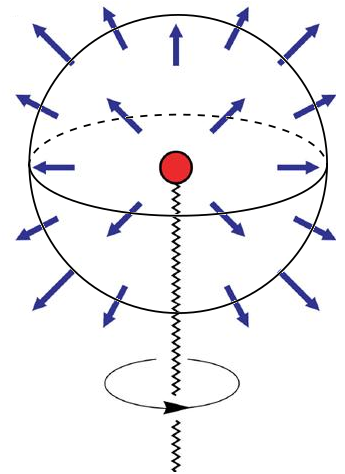
\includegraphics[scale=0.3]{DiracMon.png}
\caption{A schematization of Dirac string}
\label{fig-DirMon}
\end{figure}

\subsection{Angular momentum conservation}
Let $L$ be now the orbital angular momentum of a rotating particle with mass $m$ and charge $e$. The particle experiments a variation of $L^i=\epsilon^{ijk}r_jm\dot r_k$, such that
\begin{align}
\frac{dL^i}{dt}=\epsilon^{ijk}r_jm\ddot r_k=\epsilon^{ijk}r_j\epsilon^{klm}e\dot r_lB_m=\epsilon^{ijk}r_j\epsilon^{klm}e\dot r_l\frac{g}{4\pi r^3}B_m=\frac{d}{dt}\left(\frac{egr^i}{4\pi r}\right).
\end{align}
This implies that a particle into the monopular field conservs another quantity that is the whole momentum
\begin{equation}
J^i=L^i-\frac{egr^i}{4\pi r}.
\end{equation}
\subsection{Witten Effect}
Now we want to generalize quantization that are deduced from a generic gauge transformation about a direction $\vec\phi$. In this case we have that variations of a generic isovector $\vec v$ and vector potential $\vec A_\mu$ are
\begin{align}
&\delta\vec v=\frac{\vec\phi\times\vec v}{a}\nonumber\\
&\delta\vec A_\mu=-\frac{D_\mu\vec\phi}{ea},
\end{align}
where we have the normalization constant $a$, the electric charge $e$ and where we defined the covariant derivative
\begin{equation}
D_\mu\vec\phi=\partial_\mu\vec\phi-e\vec A_\mu\times\vec\phi.
\end{equation}
Considering now the operator $e^{2\pi i N}$, where $N$ is the same operator with Higgs solution that will be defined in the next section. In the vacuum $D_\mu\vec\phi=0$ and at infinity in space we have that this operator is equal to identity. Using the variations defined above, we can obtain the Noether charge of the related transformations, which is for $\delta\vec\phi=0$
\begin{equation}
N=-\int_{\mathcal{R}^3}\frac{1}{ae}\frac{\partial\mathcal{L}}{\partial\partial_0\vec A_i}\cdot D_i\phi=\frac{q}{e},
\end{equation}
where we used the fact that the conjugated momentum of $\vec A_i$ is $-\vec E_i$.
Instead, if we add a new term in the action
\begin{equation}
\mathcal{L}_\theta=\frac{e^2\theta}{64\pi^2}\epsilon^{\alpha\beta\mu\nu}\vec G_{\alpha\beta}\vec G_{\mu\nu},
\end{equation}
where $\vec G^{\alpha\beta}$ are the gauge field-strengths for $A$. In this case we have a modify of $N$ by a factor
\begin{equation}
\Delta N=-\frac{e\theta}{16\pi^2a}\int_{\mathcal{R}^3}\epsilon^{0i\alpha\beta}\vec G_{\alpha\beta}D_i\vec\phi=\frac{e\theta g}{8\pi^2},
\end{equation}
with the magnetic charge $g$. Rewriting this expression it follows, for $eg=-4\pi$ (the t' Hooft-Polyakov monopole result, which will be obtained later)\begin{equation}
q=ne+\frac{e\theta}{2\pi},
\end{equation}
with $n\in\mathbf{Z}$. This is the generalization to have consistency with quantization condition, a result by Edward Witten \cite{Witten}.
\end{document}